\let\negmedspace\undefined
\let\negthickspace\undefined
\documentclass[journal]{IEEEtran}
\usepackage[a4paper, margin=10mm, onecolumn]{geometry}
%\usepackage{lmodern} % Ensure lmodern is loaded for pdflatex
\usepackage{tfrupee} % Include tfrupee package

\setlength{\headheight}{1cm} % Set the height of the header box
\setlength{\headsep}{0mm}  % Set the distance between the header box and the top of the text

\usepackage{gvv-book}
\usepackage{gvv}
\usepackage{cite}
\usepackage{amsmath,amssymb,amsfonts,amsthm}
\usepackage{algorithmic}
\usepackage{graphicx}
\usepackage{float}
\usepackage{textcomp}
\usepackage{xcolor}
\usepackage{txfonts}
\usepackage{listings}
\usepackage{enumitem}
\usepackage{mathtools}
\usepackage{gensymb}
\usepackage{comment}
\usepackage[breaklinks=true]{hyperref}
\usepackage{tkz-euclide} 
\usepackage{listings}
% \usepackage{gvv}                                        
\def\inputGnumericTable{}                                 
\usepackage[latin1]{inputenc}                                
\usepackage{color}                                            
\usepackage{array}                                            
\usepackage{longtable}                                       
\usepackage{calc}                                             
\usepackage{multirow}                                         
\usepackage{hhline}                                           
\usepackage{ifthen}                                           
\usepackage{lscape}
\usepackage{tikz}
\usetikzlibrary{patterns}

\begin{document}

\bibliographystyle{IEEEtran}
\vspace{3cm}

\title{Bonus Question}
\author{ee25btech11063-vejith}

\maketitle
% \maketitle
% \newpage
% \bigskip
{\let\newpage\relax\maketitle}
\renewcommand{\thefigure}{\theenumi}
\renewcommand{\thetable}{\theenumi}
\setlength{\intextsep}{10pt} % Space between text and floats
\textbf{Question}\\
Given 3 vectors $\Vec{A}$,$\Vec{B}$,$\Vec{C}$ are coplanar then show det($\Vec{M}$) =0 where $\Vec{M}$=($\Vec{A}$  $\Vec{B}$  $\Vec{C}$)\\
\textbf{Solution}:\\
Equation of plane through 3 coplanar points is 
\begin{align}
    \Vec{n}^T\Vec{x}=0\\
    \implies \Vec{n}^T\Vec{A}= \Vec{n}^T\Vec{B} = \Vec{n}^T\Vec{C}=0\\
    \Vec{M}=(\Vec{A} \hspace{0.5cm} \Vec{B} \hspace{0.5cm} \Vec{C})\\
    \implies \Vec{n}^T\Vec{M}=(\Vec{n}^T\Vec{A} \hspace{0.5cm}  \Vec{n}^T\Vec{B} \hspace{0.5cm} \Vec{n}^T\Vec{C})\\
    \implies \Vec{n}^T\Vec{M}=(0\hspace{0.5cm} 0 \hspace{0.5cm} 0)\\
    \implies \Vec{n}^T\Vec{M}=\Vec{0}
    \end{align}
From (6) it means $\Vec{M}$ has a non trivial vector in it$'s$ null space
\begin{align}
    \implies \text{rank}(\Vec{M})<3.
\end{align}

For a 3$\times$ 3  square matrix like $\Vec{M}$ if det($\Vec{M}$)$\neq$0 means $\Vec{M}$ is invertible which means $\Vec{M}$ is a full rank matrix\\ 
$\implies$ rank($\Vec{M}$)$=$3.\brak{\text{if det($\Vec{M}$)$\neq$0}}\\ 
From (7) rank($\Vec{M}$)$<$3 \\
$\implies$ $\Vec{M}$ is not invertible\\
$\implies$ det($\Vec{M}$)$=$0\\ \\ \\  \\
\textbf{proof 2}:\\
 3 vectors $\Vec{A}$,$\Vec{B}$,$\Vec{C}$ are coplanar means they are linearly dependent.\\
 let$'$s assume
 \begin{align}
     \Vec{C}=\alpha \Vec{A}+\beta \Vec{B}.\\
     \text{det}(\Vec{M})=\text{det}((\Vec{A} \hspace{0.5cm} \Vec{B} \hspace{0.5cm} \Vec{C})\\
 =\text{det}((\Vec{A} \hspace{0.5cm} \Vec{B} \hspace{0.5cm} \alpha \Vec{A}+\beta \Vec{B})\\
 =\alpha \text{det}((\Vec{A} \hspace{0.5cm} \Vec{B} \hspace{0.5cm} \Vec{A}) + \beta \text{det}((\Vec{A} \hspace{0.5cm} \Vec{B} \hspace{0.5cm} \Vec{B})=0\\
 \implies \text{det}(\Vec{M})=0
 \end{align}

\begin{figure}[H]
    \centering
    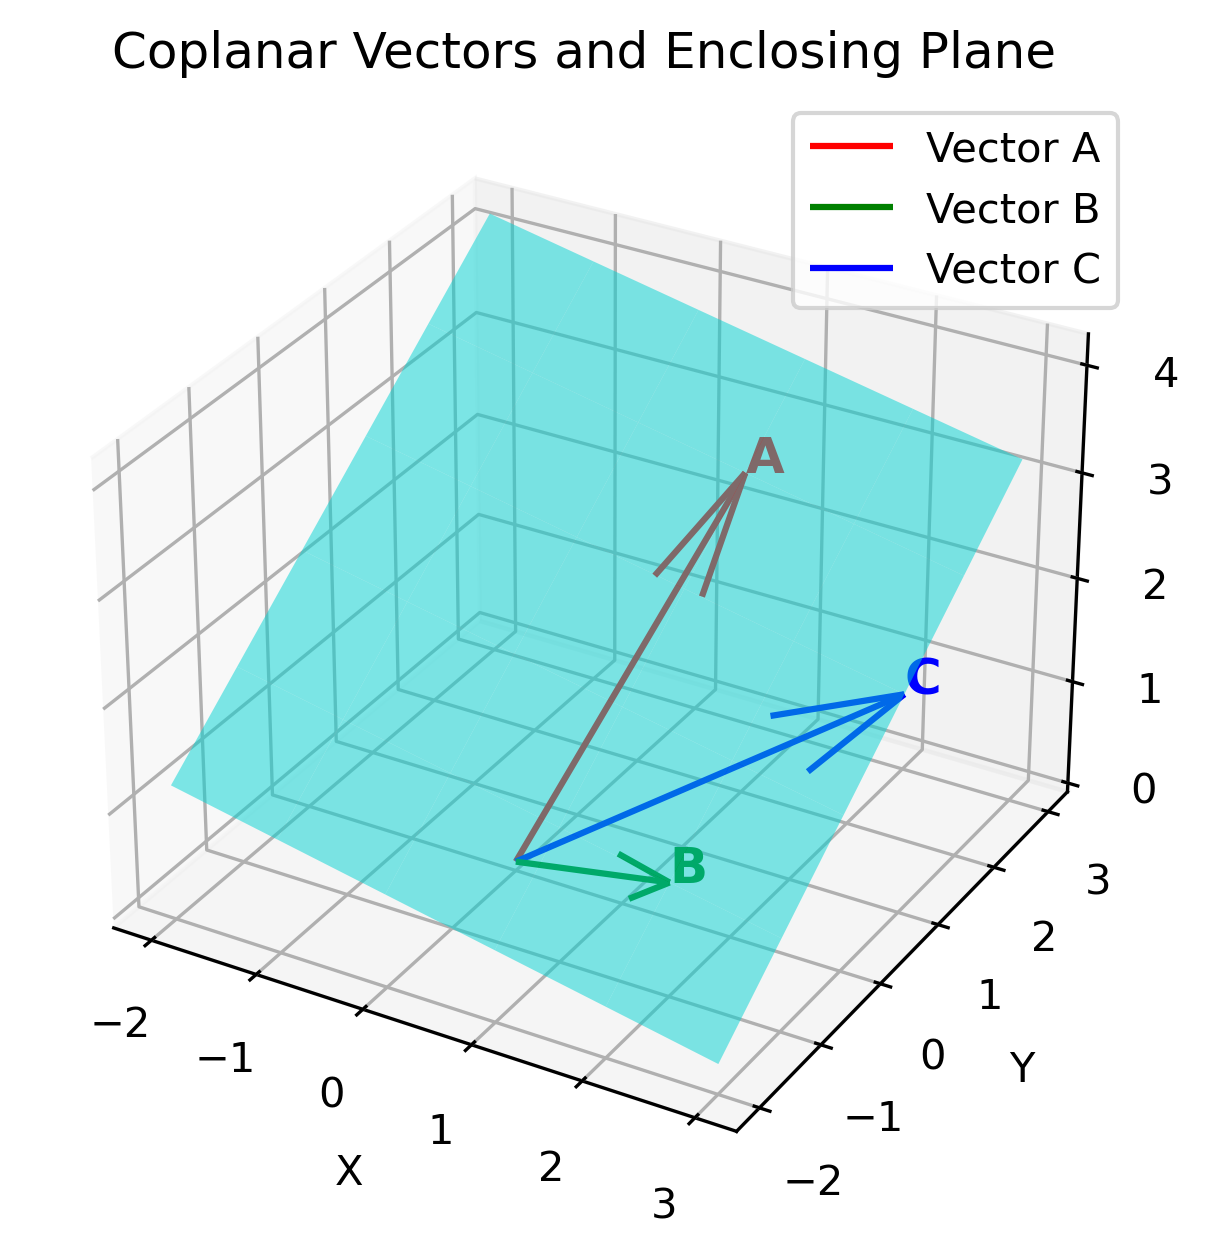
\includegraphics[width=0.50\columnwidth]{figs/01.png}
    \label{fig-1}
\end{figure}
\end{document}
